% Options for packages loaded elsewhere
\PassOptionsToPackage{unicode}{hyperref}
\PassOptionsToPackage{hyphens}{url}
\PassOptionsToPackage{dvipsnames,svgnames,x11names}{xcolor}
%
\documentclass[
  letterpaper,
  DIV=11,
  numbers=noendperiod]{scrartcl}

\usepackage{amsmath,amssymb}
\usepackage{lmodern}
\usepackage{iftex}
\ifPDFTeX
  \usepackage[T1]{fontenc}
  \usepackage[utf8]{inputenc}
  \usepackage{textcomp} % provide euro and other symbols
\else % if luatex or xetex
  \usepackage{unicode-math}
  \defaultfontfeatures{Scale=MatchLowercase}
  \defaultfontfeatures[\rmfamily]{Ligatures=TeX,Scale=1}
\fi
% Use upquote if available, for straight quotes in verbatim environments
\IfFileExists{upquote.sty}{\usepackage{upquote}}{}
\IfFileExists{microtype.sty}{% use microtype if available
  \usepackage[]{microtype}
  \UseMicrotypeSet[protrusion]{basicmath} % disable protrusion for tt fonts
}{}
\makeatletter
\@ifundefined{KOMAClassName}{% if non-KOMA class
  \IfFileExists{parskip.sty}{%
    \usepackage{parskip}
  }{% else
    \setlength{\parindent}{0pt}
    \setlength{\parskip}{6pt plus 2pt minus 1pt}}
}{% if KOMA class
  \KOMAoptions{parskip=half}}
\makeatother
\usepackage{xcolor}
\setlength{\emergencystretch}{3em} % prevent overfull lines
\setcounter{secnumdepth}{5}
% Make \paragraph and \subparagraph free-standing
\ifx\paragraph\undefined\else
  \let\oldparagraph\paragraph
  \renewcommand{\paragraph}[1]{\oldparagraph{#1}\mbox{}}
\fi
\ifx\subparagraph\undefined\else
  \let\oldsubparagraph\subparagraph
  \renewcommand{\subparagraph}[1]{\oldsubparagraph{#1}\mbox{}}
\fi


\providecommand{\tightlist}{%
  \setlength{\itemsep}{0pt}\setlength{\parskip}{0pt}}\usepackage{longtable,booktabs,array}
\usepackage{calc} % for calculating minipage widths
% Correct order of tables after \paragraph or \subparagraph
\usepackage{etoolbox}
\makeatletter
\patchcmd\longtable{\par}{\if@noskipsec\mbox{}\fi\par}{}{}
\makeatother
% Allow footnotes in longtable head/foot
\IfFileExists{footnotehyper.sty}{\usepackage{footnotehyper}}{\usepackage{footnote}}
\makesavenoteenv{longtable}
\usepackage{graphicx}
\makeatletter
\def\maxwidth{\ifdim\Gin@nat@width>\linewidth\linewidth\else\Gin@nat@width\fi}
\def\maxheight{\ifdim\Gin@nat@height>\textheight\textheight\else\Gin@nat@height\fi}
\makeatother
% Scale images if necessary, so that they will not overflow the page
% margins by default, and it is still possible to overwrite the defaults
% using explicit options in \includegraphics[width, height, ...]{}
\setkeys{Gin}{width=\maxwidth,height=\maxheight,keepaspectratio}
% Set default figure placement to htbp
\makeatletter
\def\fps@figure{htbp}
\makeatother
\newlength{\cslhangindent}
\setlength{\cslhangindent}{1.5em}
\newlength{\csllabelwidth}
\setlength{\csllabelwidth}{3em}
\newlength{\cslentryspacingunit} % times entry-spacing
\setlength{\cslentryspacingunit}{\parskip}
\newenvironment{CSLReferences}[2] % #1 hanging-ident, #2 entry spacing
 {% don't indent paragraphs
  \setlength{\parindent}{0pt}
  % turn on hanging indent if param 1 is 1
  \ifodd #1
  \let\oldpar\par
  \def\par{\hangindent=\cslhangindent\oldpar}
  \fi
  % set entry spacing
  \setlength{\parskip}{#2\cslentryspacingunit}
 }%
 {}
\usepackage{calc}
\newcommand{\CSLBlock}[1]{#1\hfill\break}
\newcommand{\CSLLeftMargin}[1]{\parbox[t]{\csllabelwidth}{#1}}
\newcommand{\CSLRightInline}[1]{\parbox[t]{\linewidth - \csllabelwidth}{#1}\break}
\newcommand{\CSLIndent}[1]{\hspace{\cslhangindent}#1}

\usepackage{booktabs}
\usepackage{longtable}
\usepackage{array}
\usepackage{multirow}
\usepackage{wrapfig}
\usepackage{float}
\usepackage{colortbl}
\usepackage{pdflscape}
\usepackage{tabu}
\usepackage{threeparttable}
\usepackage{threeparttablex}
\usepackage[normalem]{ulem}
\usepackage{makecell}
\usepackage{xcolor}
\usepackage{siunitx}

  \newcolumntype{d}{S[
    input-open-uncertainty=,
    input-close-uncertainty=,
    parse-numbers = false,
    table-align-text-pre=false,
    table-align-text-post=false
  ]}
  
\KOMAoption{captions}{tableheading}
\makeatletter
\makeatother
\makeatletter
\makeatother
\makeatletter
\@ifpackageloaded{caption}{}{\usepackage{caption}}
\AtBeginDocument{%
\ifdefined\contentsname
  \renewcommand*\contentsname{Table of contents}
\else
  \newcommand\contentsname{Table of contents}
\fi
\ifdefined\listfigurename
  \renewcommand*\listfigurename{List of Figures}
\else
  \newcommand\listfigurename{List of Figures}
\fi
\ifdefined\listtablename
  \renewcommand*\listtablename{List of Tables}
\else
  \newcommand\listtablename{List of Tables}
\fi
\ifdefined\figurename
  \renewcommand*\figurename{Figure}
\else
  \newcommand\figurename{Figure}
\fi
\ifdefined\tablename
  \renewcommand*\tablename{Table}
\else
  \newcommand\tablename{Table}
\fi
}
\@ifpackageloaded{float}{}{\usepackage{float}}
\floatstyle{ruled}
\@ifundefined{c@chapter}{\newfloat{codelisting}{h}{lop}}{\newfloat{codelisting}{h}{lop}[chapter]}
\floatname{codelisting}{Listing}
\newcommand*\listoflistings{\listof{codelisting}{List of Listings}}
\makeatother
\makeatletter
\@ifpackageloaded{caption}{}{\usepackage{caption}}
\@ifpackageloaded{subcaption}{}{\usepackage{subcaption}}
\makeatother
\makeatletter
\@ifpackageloaded{tcolorbox}{}{\usepackage[many]{tcolorbox}}
\makeatother
\makeatletter
\@ifundefined{shadecolor}{\definecolor{shadecolor}{rgb}{.97, .97, .97}}
\makeatother
\makeatletter
\makeatother
\ifLuaTeX
  \usepackage{selnolig}  % disable illegal ligatures
\fi
\IfFileExists{bookmark.sty}{\usepackage{bookmark}}{\usepackage{hyperref}}
\IfFileExists{xurl.sty}{\usepackage{xurl}}{} % add URL line breaks if available
\urlstyle{same} % disable monospaced font for URLs
\hypersetup{
  pdftitle={My title},
  pdfauthor={First author; Another author},
  colorlinks=true,
  linkcolor={blue},
  filecolor={Maroon},
  citecolor={Blue},
  urlcolor={Blue},
  pdfcreator={LaTeX via pandoc}}

\title{My title\thanks{Code and data are available at: LINK.}}
\usepackage{etoolbox}
\makeatletter
\providecommand{\subtitle}[1]{% add subtitle to \maketitle
  \apptocmd{\@title}{\par {\large #1 \par}}{}{}
}
\makeatother
\subtitle{My subtitle if needed}
\author{First author \and Another author}
\date{January 23, 2024}

\begin{document}
\maketitle
\begin{abstract}
First sentence. Second sentence. Third sentence. Fourth sentence.
\end{abstract}
\ifdefined\Shaded\renewenvironment{Shaded}{\begin{tcolorbox}[frame hidden, sharp corners, breakable, interior hidden, boxrule=0pt, borderline west={3pt}{0pt}{shadecolor}, enhanced]}{\end{tcolorbox}}\fi

\hypertarget{introduction}{%
\section{Introduction}\label{introduction}}

You can and should cross-reference sections and sub-sections.

The remainder of this paper is structured as follows.
Section~\ref{sec-data}\ldots.

\hypertarget{sec-data}{%
\section{Data}\label{sec-data}}

Some of our data is of penguins (Figure~\ref{fig-bills}), from Horst,
Hill, and Gorman (2020).

\begin{figure}

{\centering 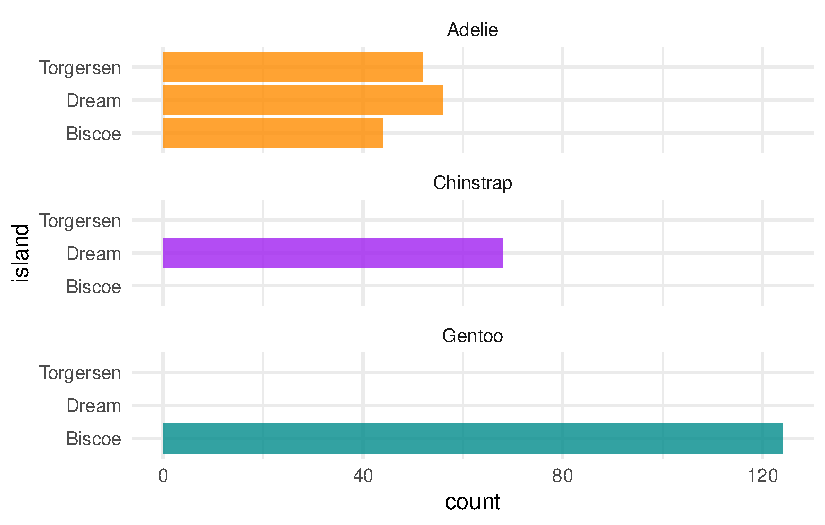
\includegraphics{paper_files/figure-pdf/fig-bills-1.pdf}

}

\caption{\label{fig-bills}Bills of penguins}

\end{figure}

Talk more about it.

And also planes (Figure~\ref{fig-planes}). (You can change the height
and width, but don't worry about doing that until you have finished
every other aspect of the paper - Quarto will try to make it look nice
and the defaults usually work well once you have enough text.)

\begin{figure}

{\centering 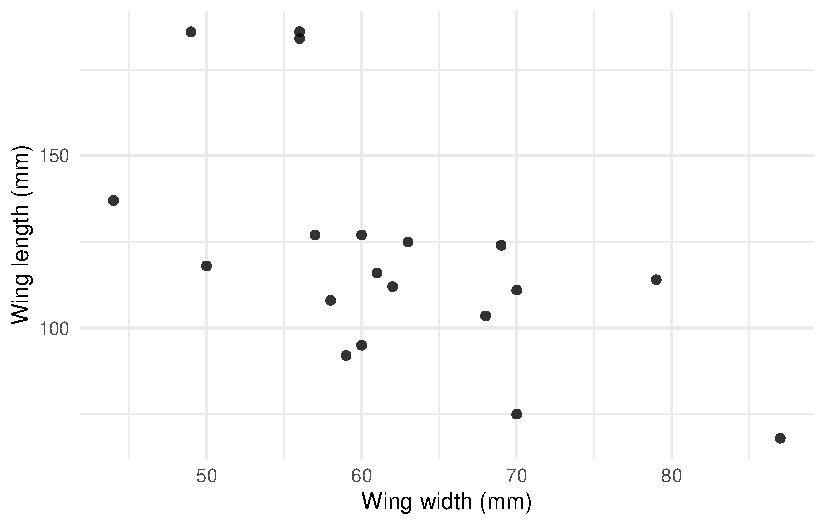
\includegraphics{paper_files/figure-pdf/fig-planes-1.pdf}

}

\caption{\label{fig-planes}Relationship between wing length and width}

\end{figure}

Talk way more about it.

\hypertarget{model}{%
\section{Model}\label{model}}

The goal of our modelling strategy is twofold. Firstly,\ldots{}

Here we briefly describe the Bayesian analysis model used to
investigate\ldots{} Background details and diagnostics are included in
Appendix~\ref{sec-model-details}.

\hypertarget{model-set-up}{%
\subsection{Model set-up}\label{model-set-up}}

Define \(y_i\) as the number of seconds that the plane remained aloft.
Then \(\beta_i\) is the wing width and \(\gamma_i\) is the wing length,
both measured in millimeters.

\begin{align} 
y_i|\mu_i, \sigma &\sim \mbox{Normal}(\mu_i, \sigma) \\
\mu_i &= \alpha + \beta_i + \gamma_i\\
\alpha &\sim \mbox{Normal}(0, 2.5) \\
\beta &\sim \mbox{Normal}(0, 2.5) \\
\gamma &\sim \mbox{Normal}(0, 2.5) \\
\sigma &\sim \mbox{Exponential}(1)
\end{align}

We run the model in R (R Core Team 2022) using the \texttt{rstanarm}
package of Goodrich et al. (2022). We use the default priors from
\texttt{rstanarm}.

\hypertarget{model-justification}{%
\subsubsection{Model justification}\label{model-justification}}

We expect a positive relationship between the size of the wings and time
spent aloft. In particular\ldots{}

We can use maths by including latex between dollar signs, for instance
\(\theta\).

\hypertarget{results}{%
\section{Results}\label{results}}

Our results are summarized in Table~\ref{tbl-modelresults}.

\hypertarget{tbl-modelresults}{}
\begin{table}
\caption{\label{tbl-modelresults}Explanatory models of flight time based on wing width and wing length }\tabularnewline

\centering
\begin{tabular}[t]{lc}
\toprule
  & First model\\
\midrule
(Intercept) & \num{1.12}\\
 & (\num{1.70})\\
length & \num{0.01}\\
 & (\num{0.01})\\
width & \num{-0.01}\\
 & (\num{0.02})\\
\midrule
Num.Obs. & \num{19}\\
R2 & \num{0.320}\\
R2 Adj. & \num{0.019}\\
Log.Lik. & \num{-18.128}\\
ELPD & \num{-21.6}\\
ELPD s.e. & \num{2.1}\\
LOOIC & \num{43.2}\\
LOOIC s.e. & \num{4.3}\\
WAIC & \num{42.7}\\
RMSE & \num{0.60}\\
\bottomrule
\end{tabular}
\end{table}

\hypertarget{discussion}{%
\section{Discussion}\label{discussion}}

\hypertarget{sec-first-point}{%
\subsection{First discussion point}\label{sec-first-point}}

If my paper were 10 pages, then should be be at least 2.5 pages. The
discussion is a chance to show off what you know and what you learnt
from all this.

\hypertarget{second-discussion-point}{%
\subsection{Second discussion point}\label{second-discussion-point}}

\hypertarget{third-discussion-point}{%
\subsection{Third discussion point}\label{third-discussion-point}}

\hypertarget{weaknesses-and-next-steps}{%
\subsection{Weaknesses and next steps}\label{weaknesses-and-next-steps}}

Weaknesses and next steps should also be included.

\newpage

\appendix

\hypertarget{appendix}{%
\section*{Appendix}\label{appendix}}
\addcontentsline{toc}{section}{Appendix}

\hypertarget{additional-data-details}{%
\section{Additional data details}\label{additional-data-details}}

\hypertarget{sec-model-details}{%
\section{Model details}\label{sec-model-details}}

\hypertarget{posterior-predictive-check}{%
\subsection{Posterior predictive
check}\label{posterior-predictive-check}}

In Figure~\ref{fig-ppcheckandposteriorvsprior-1} we implement a
posterior predictive check. This shows\ldots{}

In Figure~\ref{fig-ppcheckandposteriorvsprior-2} we compare the
posterior with the prior. This shows\ldots{}

\begin{figure}

\begin{minipage}[t]{0.50\linewidth}

{\centering 

\raisebox{-\height}{

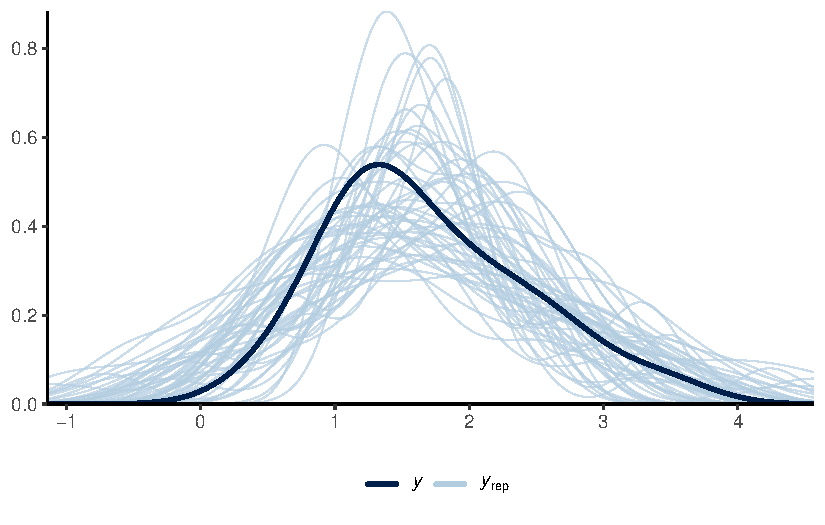
\includegraphics{paper_files/figure-pdf/fig-ppcheckandposteriorvsprior-1.pdf}

}

}

\subcaption{\label{fig-ppcheckandposteriorvsprior-1}Posterior prediction
check}
\end{minipage}%
%
\begin{minipage}[t]{0.50\linewidth}

{\centering 

\raisebox{-\height}{

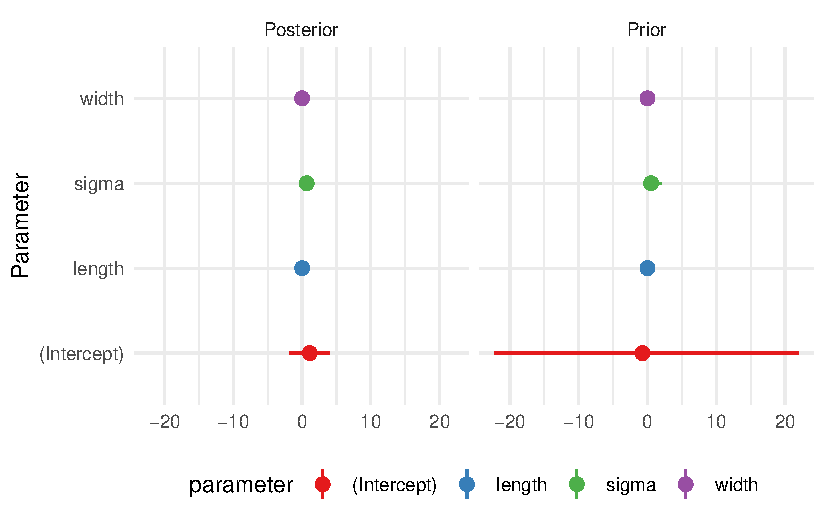
\includegraphics{paper_files/figure-pdf/fig-ppcheckandposteriorvsprior-2.pdf}

}

}

\subcaption{\label{fig-ppcheckandposteriorvsprior-2}Comparing the
posterior with the prior}
\end{minipage}%

\caption{\label{fig-ppcheckandposteriorvsprior}Examining how the model
fits, and is affected by, the data}

\end{figure}

\hypertarget{diagnostics}{%
\subsection{Diagnostics}\label{diagnostics}}

Figure~\ref{fig-stanareyouokay-1} is a trace plot. It shows\ldots{} This
suggests\ldots{}

Figure~\ref{fig-stanareyouokay-2} is a Rhat plot. It shows\ldots{} This
suggests\ldots{}

\begin{figure}

\begin{minipage}[t]{0.50\linewidth}

{\centering 

\raisebox{-\height}{

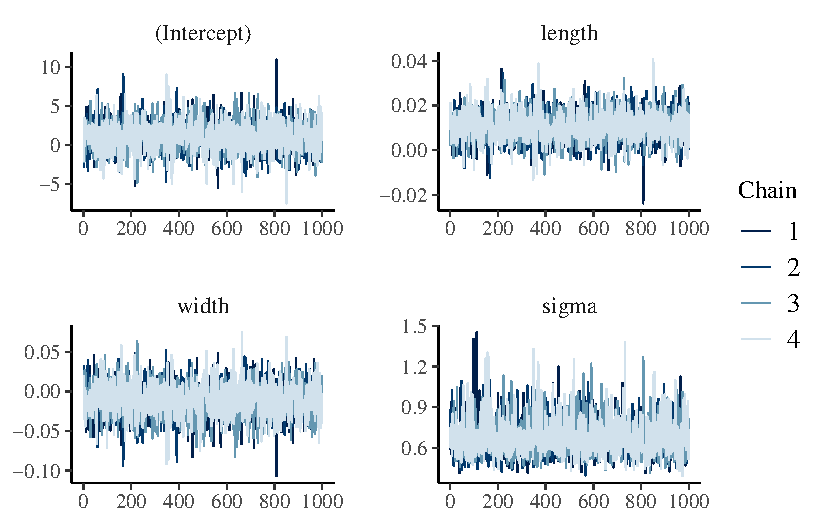
\includegraphics{paper_files/figure-pdf/fig-stanareyouokay-1.pdf}

}

}

\subcaption{\label{fig-stanareyouokay-1}Trace plot}
\end{minipage}%
%
\begin{minipage}[t]{0.50\linewidth}

{\centering 

\raisebox{-\height}{

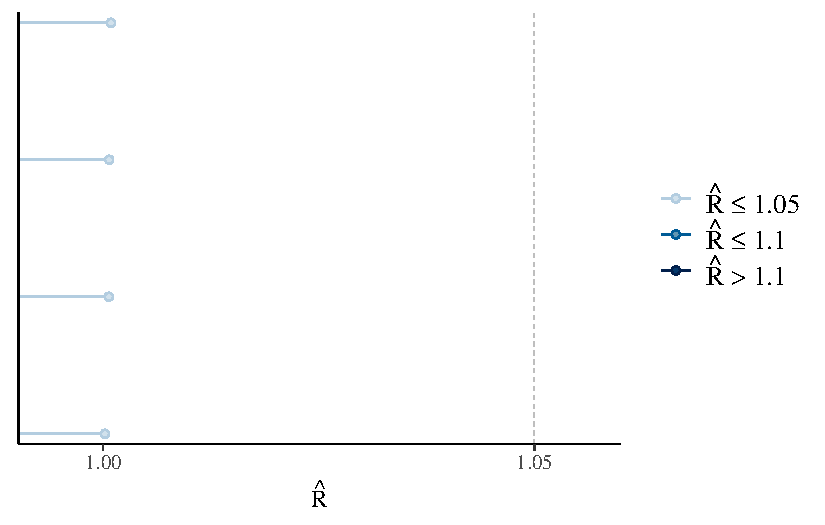
\includegraphics{paper_files/figure-pdf/fig-stanareyouokay-2.pdf}

}

}

\subcaption{\label{fig-stanareyouokay-2}Rhat plot}
\end{minipage}%

\caption{\label{fig-stanareyouokay}Checking the convergence of the MCMC
algorithm}

\end{figure}

\newpage

\hypertarget{references}{%
\section*{References}\label{references}}
\addcontentsline{toc}{section}{References}

\hypertarget{refs}{}
\begin{CSLReferences}{1}{0}
\leavevmode\vadjust pre{\hypertarget{ref-rstanarm}{}}%
Goodrich, Ben, Jonah Gabry, Imad Ali, and Sam Brilleman. 2022.
{``Rstanarm: {Bayesian} Applied Regression Modeling via {Stan}.''}
\url{https://mc-stan.org/rstanarm/}.

\leavevmode\vadjust pre{\hypertarget{ref-palmerpenguins}{}}%
Horst, Allison Marie, Alison Presmanes Hill, and Kristen B Gorman. 2020.
\emph{Palmerpenguins: Palmer Archipelago (Antarctica) Penguin Data}.
\url{https://doi.org/10.5281/zenodo.3960218}.

\leavevmode\vadjust pre{\hypertarget{ref-citeR}{}}%
R Core Team. 2022. \emph{R: A Language and Environment for Statistical
Computing}. Vienna, Austria: R Foundation for Statistical Computing.
\url{https://www.R-project.org/}.

\end{CSLReferences}



\end{document}
